\documentclass[oneside,12pt,letterpaper]{article}

% Imports and Definitions
%% Packages
\usepackage{amsmath}
\usepackage{amsfonts}
\usepackage{amssymb}
\usepackage{amsthm}
\usepackage{arydshln}
\usepackage{color}
\usepackage{extramarks}
\usepackage{fancyhdr}
\usepackage{float}
\usepackage[margin=1in]{geometry}
\usepackage{graphicx}
\usepackage{listings}
\usepackage{multicol}
\usepackage{setspace}
\usepackage{subcaption}
\usepackage{textcomp}
\usepackage{url}
\usepackage{xspace}
\usepackage{mathtools}

%% Commands
%%% Metadata
\newcommand{\metaTitle}{Comprehensive Exam}
\newcommand{\metaDueDate}{November 24, 2020}
\newcommand{\metaDueTime}{04:00 PM}
\newcommand{\metaSchool}{IUPUI}
\newcommand{\metaClass}{STAT 52400}
\newcommand{\metaDepartment}{Statistics Department}
\newcommand{\metaAuthorName}{Ross Grinvalds}

%%% Aliases
\newcommand{\Bias}{\mathrm{Bias}}
\newcommand{\Cov}{\mathrm{Cov}}
\newcommand{\dd}[1]{\frac{\mathrm{d}}{\mathrm{d}x} (#1)}
\newcommand{\dx}{\mathrm{d}x}
\newcommand{\E}{\mathrm{E}}
\newcommand{\m}[1]{\begin{bmatrix*}[r]#1\end{bmatrix*}}
\newcommand{\md}[1]{\begin{vmatrix*}#1\end{vmatrix*}}
\newcommand{\mf}[1]{\mathrm{\bf{#1}}}
\newcommand{\p}[1]{\begin{pmatrix}#1\end{pmatrix}} 
\newcommand{\pdd}[2]{\frac{\partial}{\partial #1} (#2)}
\newcommand{\solution}{\textbf{\large Solution}}
\newcommand{\T}{\intercal}
\newcommand{\Var}{\mathrm{Var}}

%%% Math Functions
\makeatletter
\newsavebox{\mybox}\newsavebox{\mysim}
\newcommand{\distras}[1]{%
  \savebox{\mybox}{\hbox{\kern3pt$\scriptstyle#1$\kern3pt}}%
  \savebox{\mysim}{\hbox{$\sim$}}%
  \mathbin{\overset{#1}{\kern\z@\resizebox{\wd\mybox}{\ht\mysim}{$\sim$}}}%
}
\makeatother

\newcommand{\indep}{\perp \!\!\! \perp}

%% Environments
%%% R Code
\newcommand{\ri}[1]{\lstinline{#1}}  %% Short for 'R inline'

\lstnewenvironment{rc}[1][]{
	\lstset{commentstyle=\color{red}, keywordstyle=\color{black}, showstringspaces=true, language=R, basicstyle=\ttfamily\tiny}
}{}
\lstset{language=R}


% Settings
%% Document-wide
\pagestyle{fancy}

%% Header and Footer
\setlength{\headheight}{15pt}
\lhead{\metaAuthorName}
\chead{\metaSchool\ \metaClass:\ \metaTitle}
\rhead{\metaDepartment}
\cfoot{\thepage}

%% Title Page
\title{
	\vspace{1in}
	\textmd{\textbf{\metaSchool\ \metaClass:\ \metaTitle}}\\
	\normalsize\vspace{0.1in}\small{Due\ by\ \metaDueDate\ at \metaDueTime}\\
	\vspace{6in}
}
\author{\metaAuthorName}
\date{}


\begin{document}
\maketitle

\section*{Problem 5.1}
\begin{enumerate}
\item[\bf{a)}] Evaluate $T^2$, for testing $H_0: \vec{\mu}_0^{\intercal} = \m{7 & 11}$ using the data $$\mf{X} = \m{2 & 12 \\ 8 & 9 \\ 6 & 9 \\ 8 & 10}$$ The test statistic is defined as follows: $T^2 = n \p{\bar{\vec{x}} - \vec{\mu_0}}^{\intercal} \mf{S}^{-1} \p{\bar{\vec{x}} - \vec{\mu_0}}$. Then, calculate the necessary components piecewise to assemble the statistic.
	\begin{align*}
		\bar{\vec{x}} &= \m{\bar{x_1} \\ \bar{x_2}} = \m{6 \\ 10} \\
		s_{11} &= \frac{24}{3} \\
		s_{22} &= \frac{6}{3} \\
		s_{12} &= s_{21} = \frac{-10}{3} \\
		\implies \mf{S} &= \frac{1}{3} \m{24 & -10 \\ -10 & 6} \\
	\end{align*}
	Next, compute the test statistic.
	\begin{align*}
		T^2 &= 4 \cdot \m{-1 & -1} \frac{3}{44} \m{2 & 10 \\ 10 & 8} \m{-1 \\ -1} \\
				&= 13.636 \ldots
	\end{align*}

\item[\bf{b)}] The distribution of Hotelling's $T^2$ test statistic is an $F$ distribution with $p$ and $n-p$ degrees of freedom for the numerator and denominator, respectively. More specifically: $$T^2 \distras{} \frac{(n-1)p}{(n-p)}F_{p, n-p}$$ 

\item[\bf{c)}] Given a specified chance of Type I error denoted by $\alpha = 0.05$, the critical value of the $F^*_{p, n-p}(1-\alpha) = 19.00$. This suggests that the critical value of the Hotelling test statistic if $3 \cdot 19 = 57$. Comparing the result from $\bf{a)}$ with the critical value it is observed that $13.636 \ldots < 57$. Therefore, the data suggests that the null hypothesis should be maintained, that is, the hypothesized mean vector is supported by the data.

\end{enumerate}

\newpage
\section*{Problem 5.3}
\begin{enumerate}
\item[\bf{a)}] Use the following expression to reevaluate the Hotelling $T^2$ statistic from problem $5.1$.
	\begin{align*}
		T^2 &= \frac{(n-1)\md{\hat{\Sigma}_0}}{\md{\hat{\Sigma}}} \\
				&=\frac{(n-1)\md{\sum_{j=1}^n\p{\vec{x}_j-\vec{\mu}_0}\p{\vec{x}_j-\vec{\mu}_0}^{\intercal}}}{\md{\sum_{j=1}^n\p{\vec{x}_j-\bar{\vec{x}}}\p{\vec{x}_j-\bar{\vec{x}}}^{\intercal}}}
	\end{align*}
	The determinant of the denominator was calculated in part $\bf{5.1.a)}$, therefore, the only quantity left to compute is the determinant in the numerator. Recall that $\vec{\mu}_0 = \m{7 & 11}^{\intercal}$, then:
	\begin{align*}
		\hat{\Sigma}_0 &= \frac{1}{3} \m{28 & -6 \\ -6 & 10} \\
		\\
		\therefore T^2 &= \frac{3 \md{\frac{1}{3} \m{28 & -6 \\ -6 & 10}}}{\md{\frac{1}{3} \m{24 & -10 \\ -10 & 6}}} - 3\\
									 &= \frac{3 \cdot 244}{44} - 3 \\
									 &= 16.636 \ldots - 3 \\
									 &= 13.636 \ldots
	\end{align*}
	Which agrees with the results from problem $\bf{5.1}$.

\item[\bf{b)}] Given the data matrix $\mf{X}$ from problem $5.1$, evaluate the likelihood ratio, $\Lambda$, as well as Wilks' lambda, $\Lambda^{\frac{n}{2}}$.
	\begin{align*}
		\Lambda &= \p{\frac{\md{\hat{\Sigma}}}{\md{\hat{\Sigma}_0}}}^{\frac{n}{2}} \\
						&= \p{\frac{44}{244}}^{\frac{4}{2}} \\
						&= \p{0.180 \ldots}^2 \\
						&= 0.0325 \ldots \\
		\\
		Wilks' Lambda &= \Lambda^{\frac{2}{n}} \\
									&= 0.180...
	\end{align*}
	This calculation of Wilks' Lambda should be equivalent to the following value using Hotelling's $T^2$ statistic:
	\begin{align*}
		\Lambda^{\frac{2}{n}} &= \p{1 + \frac{T^2}{n-1}}^{-1} \\
													&= \p{1 + \frac{13.636 \ldots}{3}}^{-1} \\
													&= \frac{1}{5.545 \ldots} \\
													&= 0.180 \ldots
	\end{align*}

\end{enumerate}

\newpage
\section*{Problem 5.20}
This problem focuses on data collected on $n = 45$ female hook-billed kites. The data set is composed of two variables representing the tail length ($X_1$) and wing length ($X_2$) of the observed birds.

\begin{enumerate}
\item[\bf{a)}] A $95\%$ confidence ellipse for the mean vector, $\vec{\mu}$, was constructed given the sample. This confidence ellipse can be observed below. The suggested mean vector representing the tail length and wing length of male hook-billed kites is also plotted on the graph and is represented by a black $+$ sign. Because the point lies within the confidence interval for the female hook-billed kites, it is suggested that the mean vector for the males represent plausible values for the mean vector for the females. Simply That is, given a probability of committing a Type I Error to be $\alpha = 0.05 = 5\%$, there is no distinguishible difference between the male and female hook-billed kites' mean tail length and mean wing length given the sample data for these $45$ females.
	
	\begin{center}
		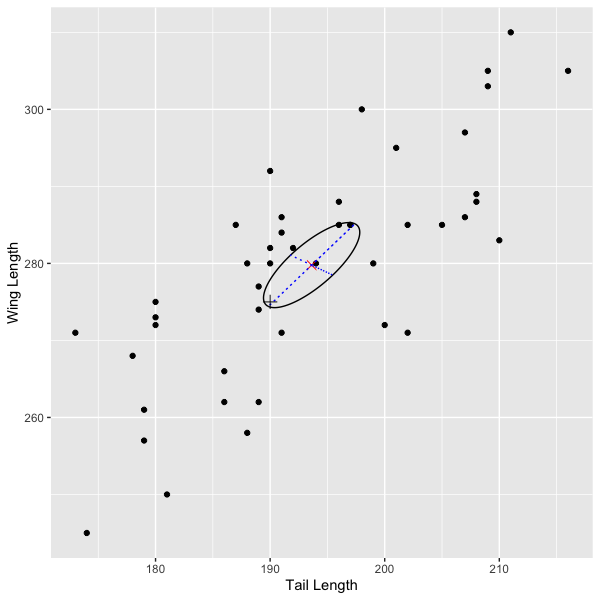
\includegraphics[width=4in]{plot_5_20_a_ellipse.png}
	\end{center}
	
Although the specified mean vector of the male kites is evident visually, were there more than three variables to consider, a numerical analysis can also be performed. The statistical distance from the sample mean to the specified vector is obtained. If this value is less than the critical value of the Hotelling $T^2$ distribution used to construct the region, it is considered 'within' the hyperellipsoid. To verify this statement for this particular case: 
\begin{align*}
	\m{\vec{x} - \bar{\vec{x}}}^{\intercal} \mf{S}^{-1} \m{\vec{x} - \bar{\vec{x}}} &<  \frac{p(n-1}{n(n-p} F_{p, n-p}^*(1-\alpha) \\
	\m{-3.622,\ -4.778}^{\intercal} \m{120.695 & 122.347 \\ 122.346 & 208.540}^{-1} \m{-3.622,\ -4.778} &< \frac{2 \cdot 44}{45 \cdot 43}F_{2, 43}^*(0.95) \\
	0.123 &< 0.146
\end{align*}
This confirms that the specified mean vector of male hook-billed kites does in fact lie within the confidence region generated by the sample.
	
\item[\bf{b)}] Next, two different $95\%$ simultaneous confidence intervals for $\mu_1$ and $\mu_2$ were generated in R given the sample data. Both intervals are centered around the sample mean values for each variable, but the margins of error vary between techniques. First, $T^2$ intervals were considered. The margin of error for the $T^2$ intervals are defined as follows: $$MOE = \sqrt{\frac{(n-1)p}{n-p}F_{p, n-p}^*(1-\alpha)} \cdot \sqrt{\frac{s_{jj}}{n}}$$ For $i = 1$: $MOE = \sqrt{6.578} \cdot \sqrt{2.682} = 4.200$. Therefore, the $95\%$ $T^2$ confidence interval for $\vec{\mu}_1$ is: $$\bar{\vec{x}}_1 \pm MOE = 193.622 \pm 4.2 = (189.421,\ 197.823)$$ Similarly, for $\vec{\mu}_2$, the $95\%$ confidence interval is: $$279.777 \pm 4.995 = (274.256,\ 285.299)$$

	Simultaneous Bonferroni confidence intervals may also be constructed using a different margin of error. These intervals are constructed from an assumedly uncorrelated structure between the variables. This leads to confidence intervals that are always equally wide or narrower than the simultaneous $T^2$ intervals. The margin of error is defined as: $$MOE = t_{n-1}^*\p{1-\frac{\alpha}{2p}} \cdot \sqrt{\frac{s_{ii}}{n}}$$ For $i = 1$: $MOE = t_{44}^*\p{0.9875} \cdot \sqrt{\frac{s_{11}}{n}} = 2.320 \cdot \sqrt{2.682} = 3.800$. Therefore, the $95\%$ simultaneous Bonferroni confidence interval for $\vec{\mu}_1$ is: $$193.622 \pm 3.8 = (189.821,\ 197.423)$$ Similarly for $\vec{\mu}_2$, the $95\%$ Bonferroni confidence interval is: $$279.777 \pm 4.996 = (274.782,\ 284.774)$$
	
	As shown above, the Bonferroni confidence intervals are indeed narrower in this case.
	
	\item[\bf{c)}] Throughout this analysis, the underlying assumption was that the joint distribution of the hook-billed kites' tail length and wing length was bivariate normal. This assumption needs to be investigated in order to suggest that the above analysis is valid. First, univariate histograms and quantile-quantile plots were generated for $X_1$ and $X_2$, see below. Both histograms exhibit symmetrically distributed observations with little to no skewness. The quantile plots are relatively linear but do suggest that there may be a multimodal distribution of $X_2$, however, there is not sufficient evidence in the visual analysis to reject the assumption of normality. Additionally, both univariate data sets were tested for normality using the Shapiro-Wilks test and correlation quantile test. These tests all supported the assumption of univariate normality. 

	\begin{center}
		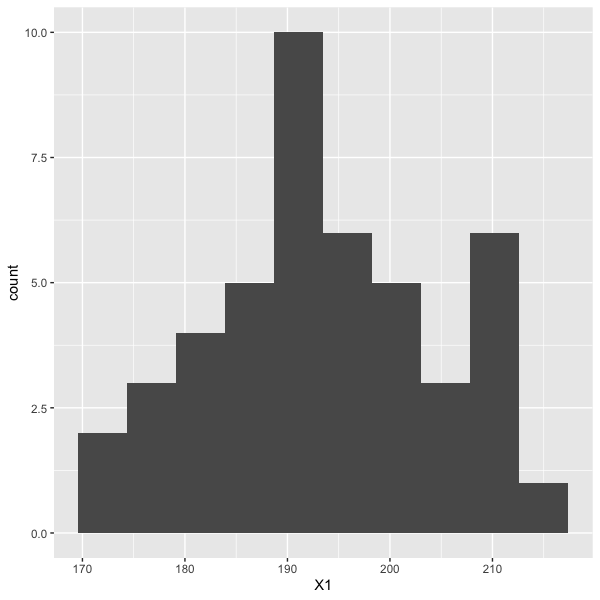
\includegraphics[width=3in]{plot_5_20_c_X1hist.png}
		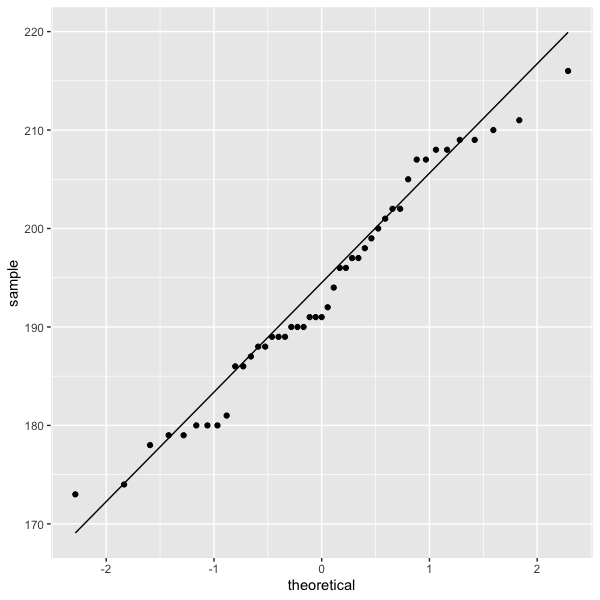
\includegraphics[width=3in]{plot_5_20_c_X1qq.png}
		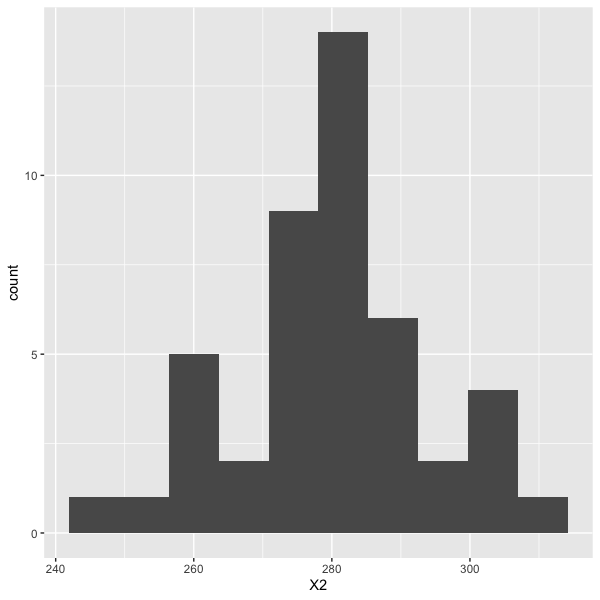
\includegraphics[width=3in]{plot_5_20_c_X2hist.png}
		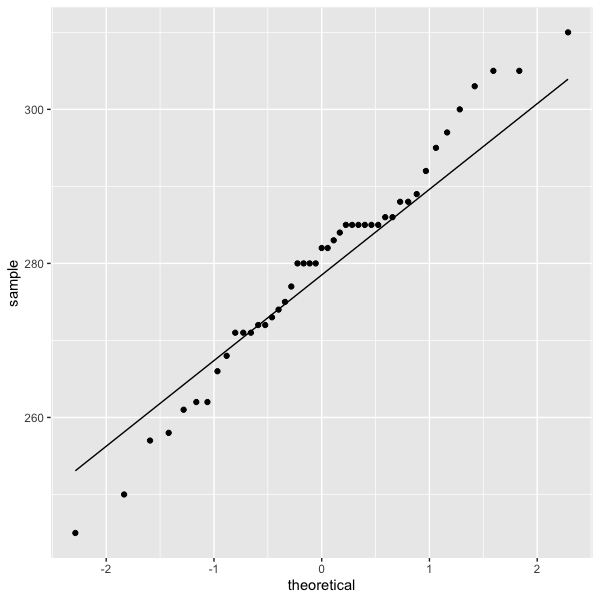
\includegraphics[width=3in]{plot_5_20_c_X2qq.png}
	\end{center}

	After the univariate normality assessment, the joint distribution was visually assessed for bivariate normality. A scatter plot with confidence ellipse bounded by the statistical distance of $\mathcal{X}_2^2(0.5)=1.386$ is used to gauge the distribution for an elliptical shape. While roughly half of the points should lie within the plotted confidence ellipse, there are only $\frac{17}{45}=0.377$. It is unclear from this proportion alone if the bivariate normality is violated, however, after an ad hoc analysis replicating the above steps throughout part $\bf{c)}$ on data transformed via the simultaneous Box-Cox method, there were no substantial differences from the analysis performed prior to transformation. Therefore, the assumption of normality should be maintained.

	\begin{center}
		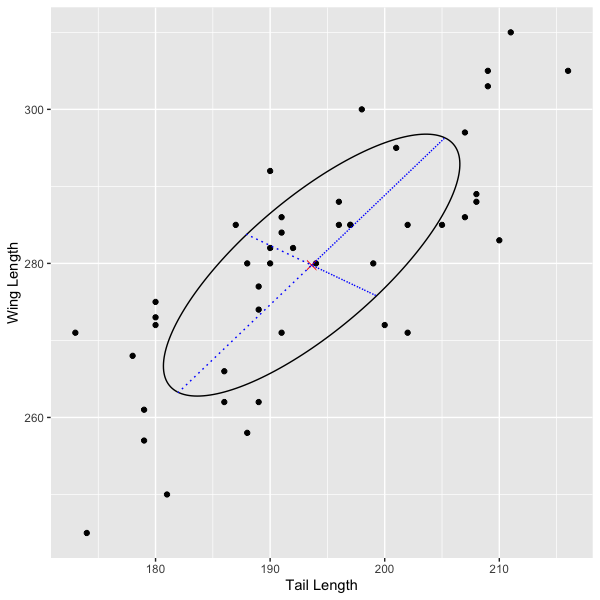
\includegraphics[width=6in]{plot_5_20_c_X1X2.png}
	\end{center}

	
\end{enumerate}


\end{document}
